\chapter{Cosas Capítulo 4} \label{apen:flageul}

\section{isoQ vs isoT}

``A efectos practicos las aproximacion de flujo de calor cte (condicion de Neuman) como una condición de Dirichlet igual a 0 resulta mejor desde el punto de vista numérico ya que la fluctuación de los campos es mayor y se requiere más tiempo de corrida para conseguir una buena estadistica ...''

\begin{figure}[H]
  \centering  
  \subfloat[]{
    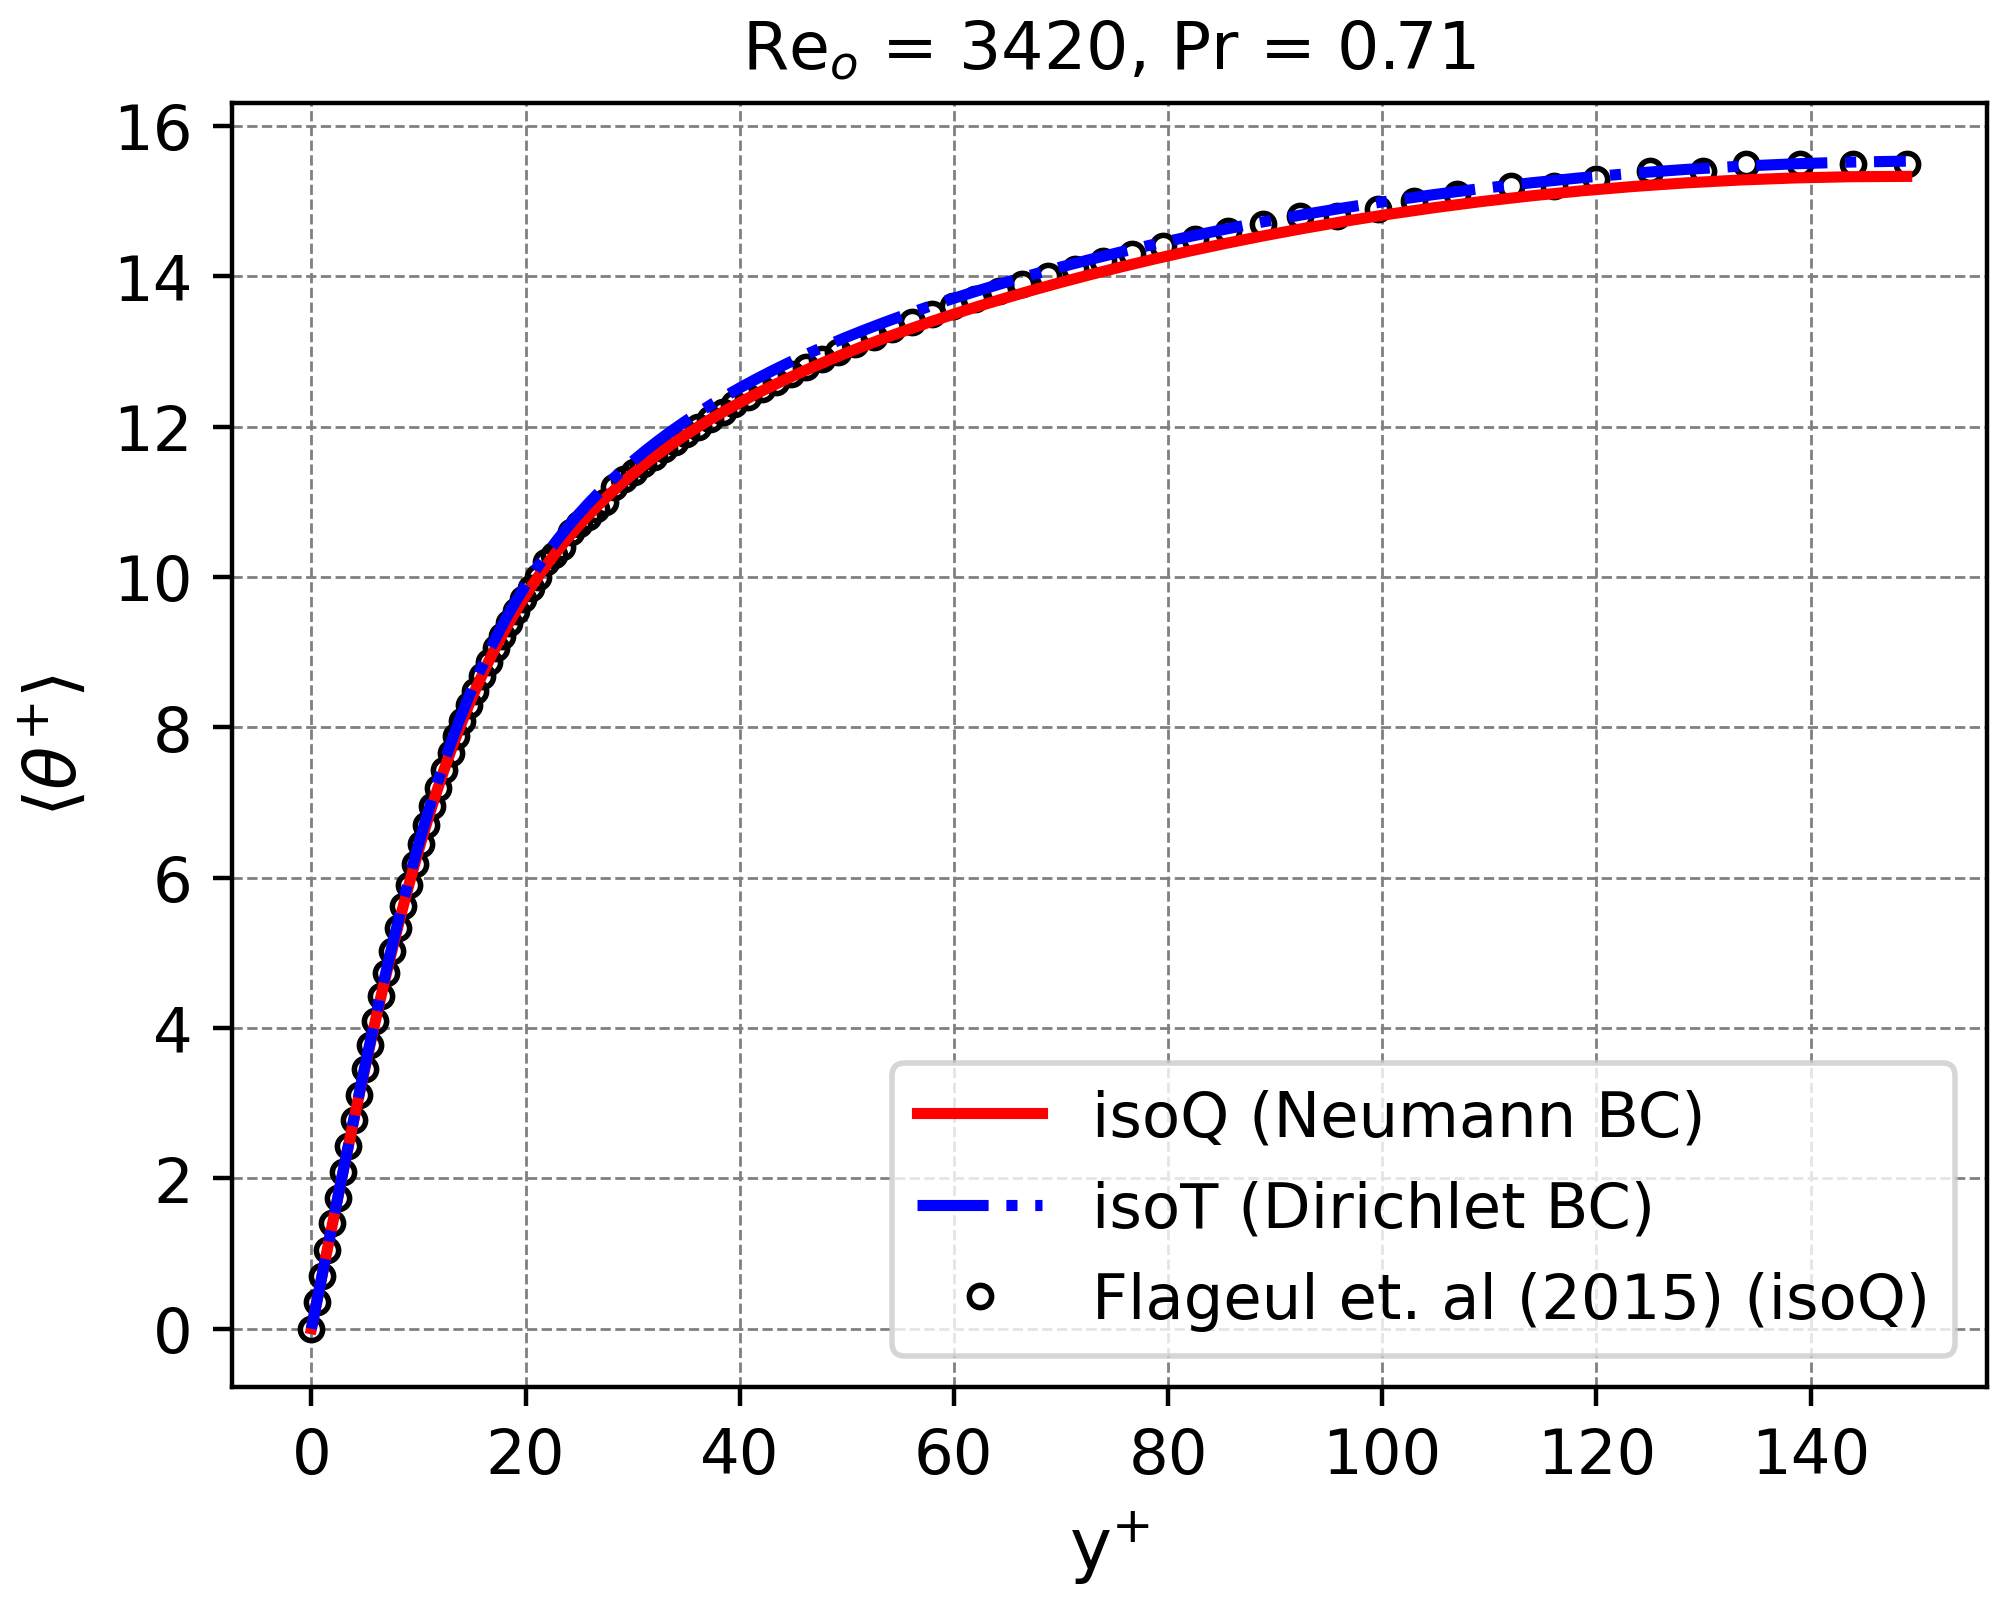
\includegraphics[width=0.49\textwidth]{figures/cap4/flageul/tep_theta.png}
    \label{fig:flageul-theta}}
  \subfloat[]{
    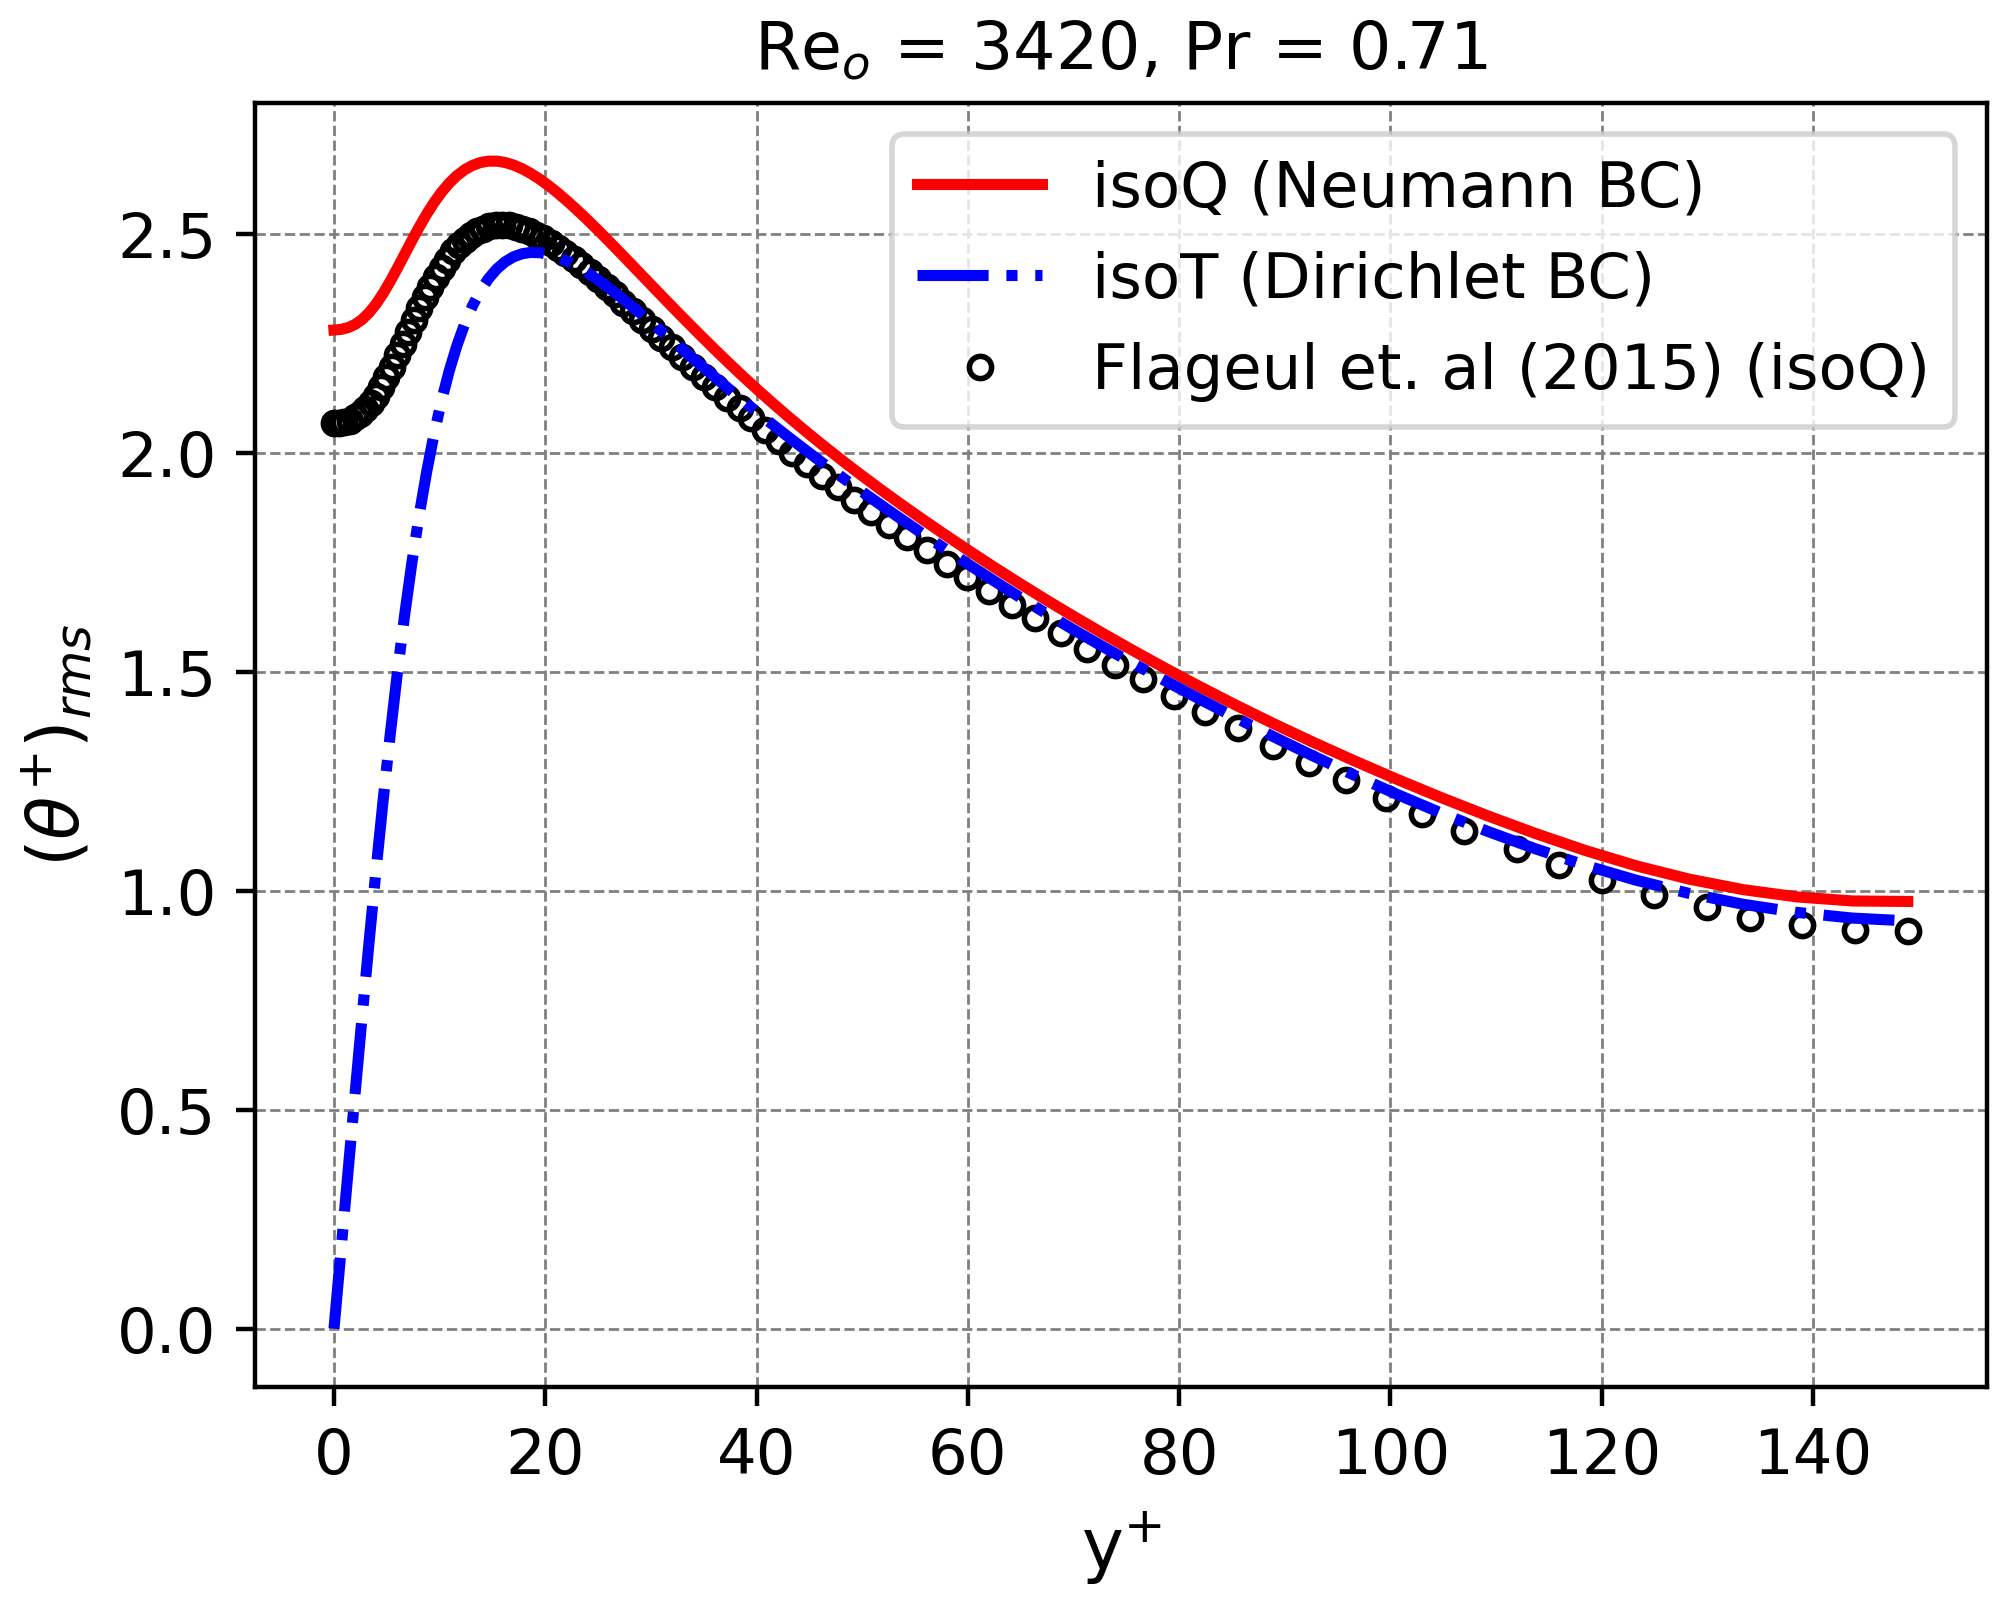
\includegraphics[width=0.49\textwidth]{figures/cap4/flageul/tep_thetap_rms.png}
    \label{fig:flageul-theta-rms}}
  \caption{}
  \label{fig:flageul}
\end{figure}

\begin{figure}[H]
  \centering  
  \subfloat[]{
    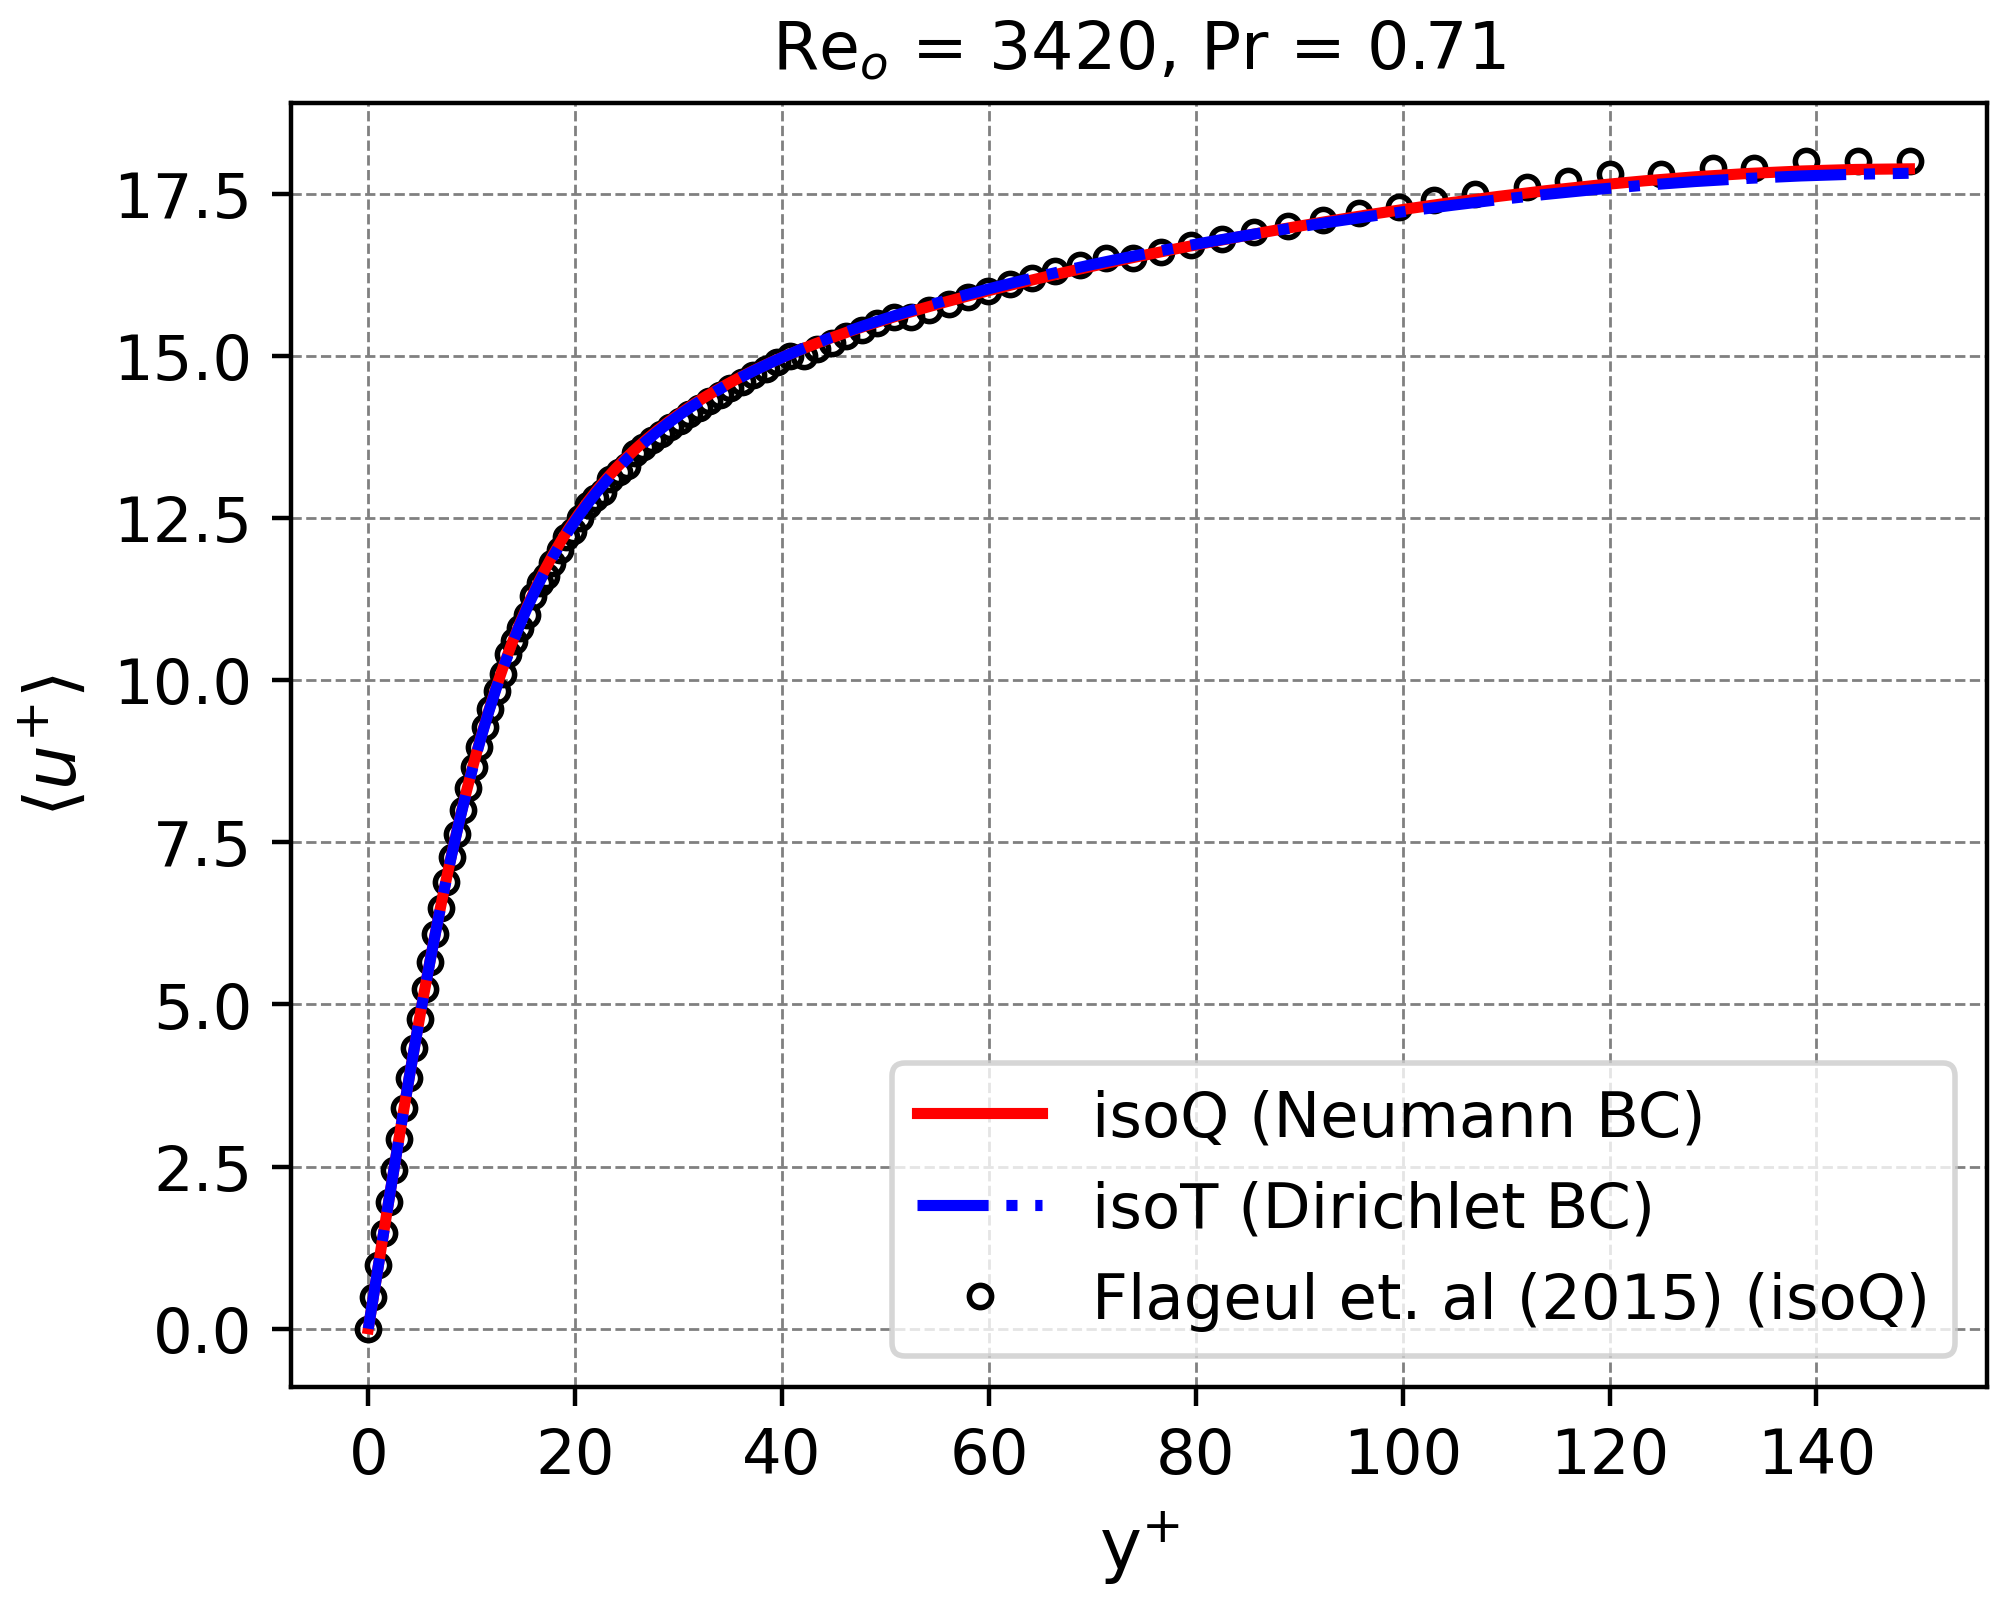
\includegraphics[width=0.49\textwidth]{figures/cap4/flageul/upmean.png}
    \label{fig:flageul-up}}
  \subfloat[]{
    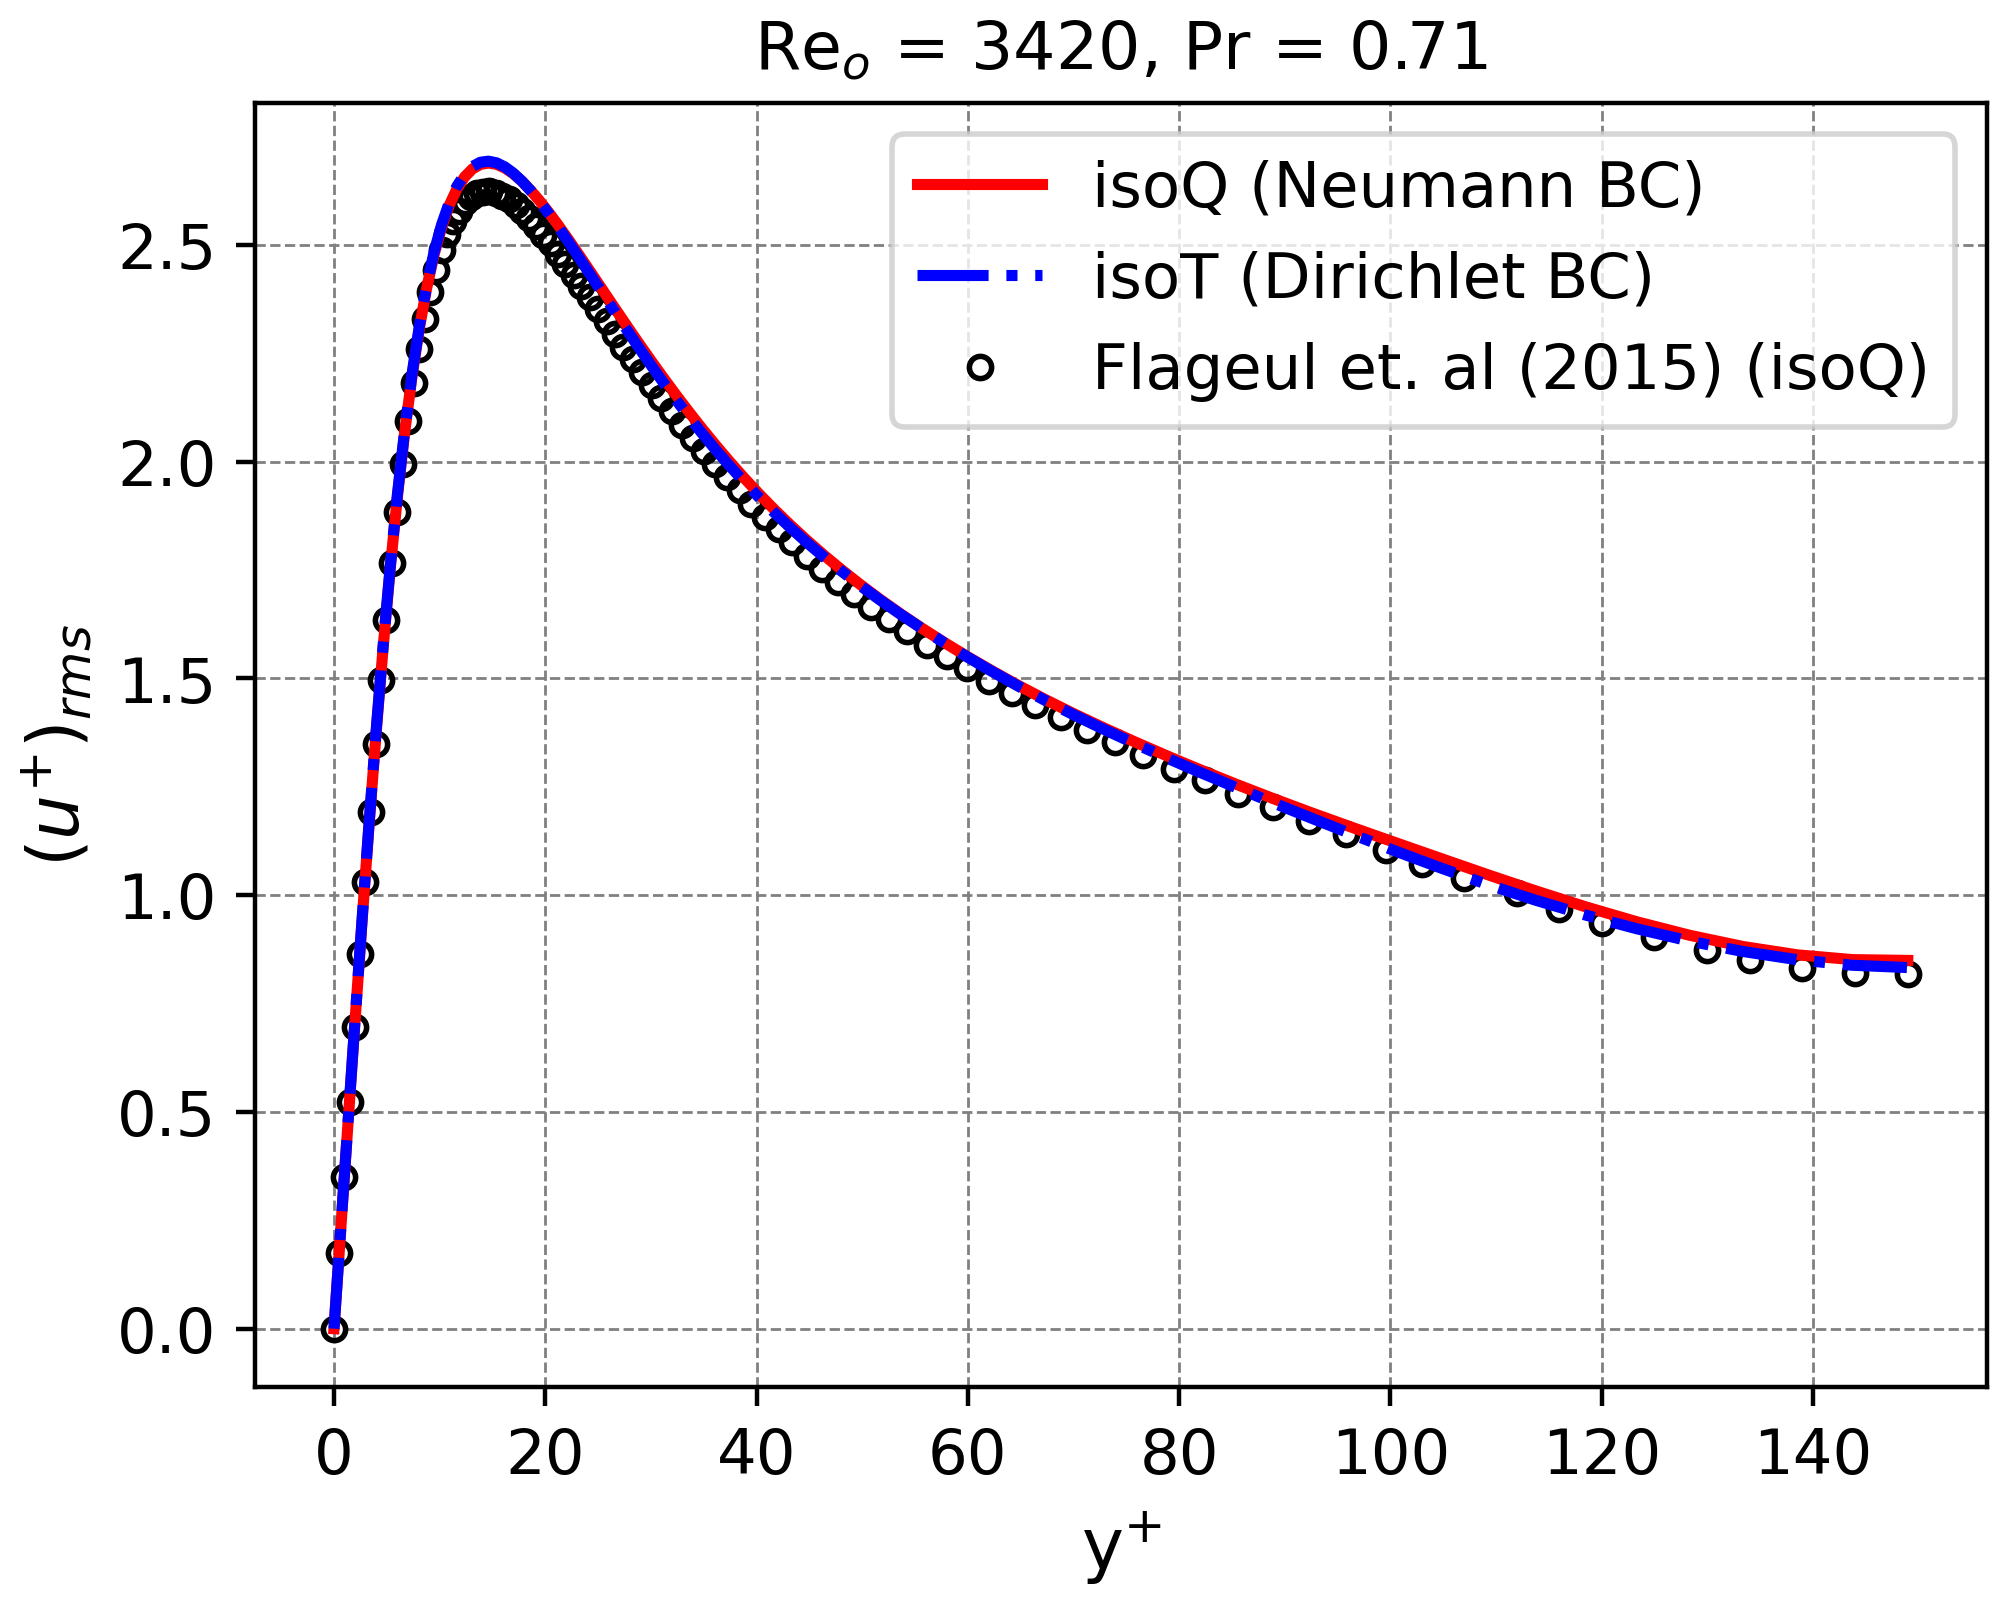
\includegraphics[width=0.49\textwidth]{figures/cap4/flageul/uprms.png}
    \label{fig:flageul-up-rms}}
  \caption{}
  \label{fig:flageul}
\end{figure}

\begin{figure}[H]
  \centering  
    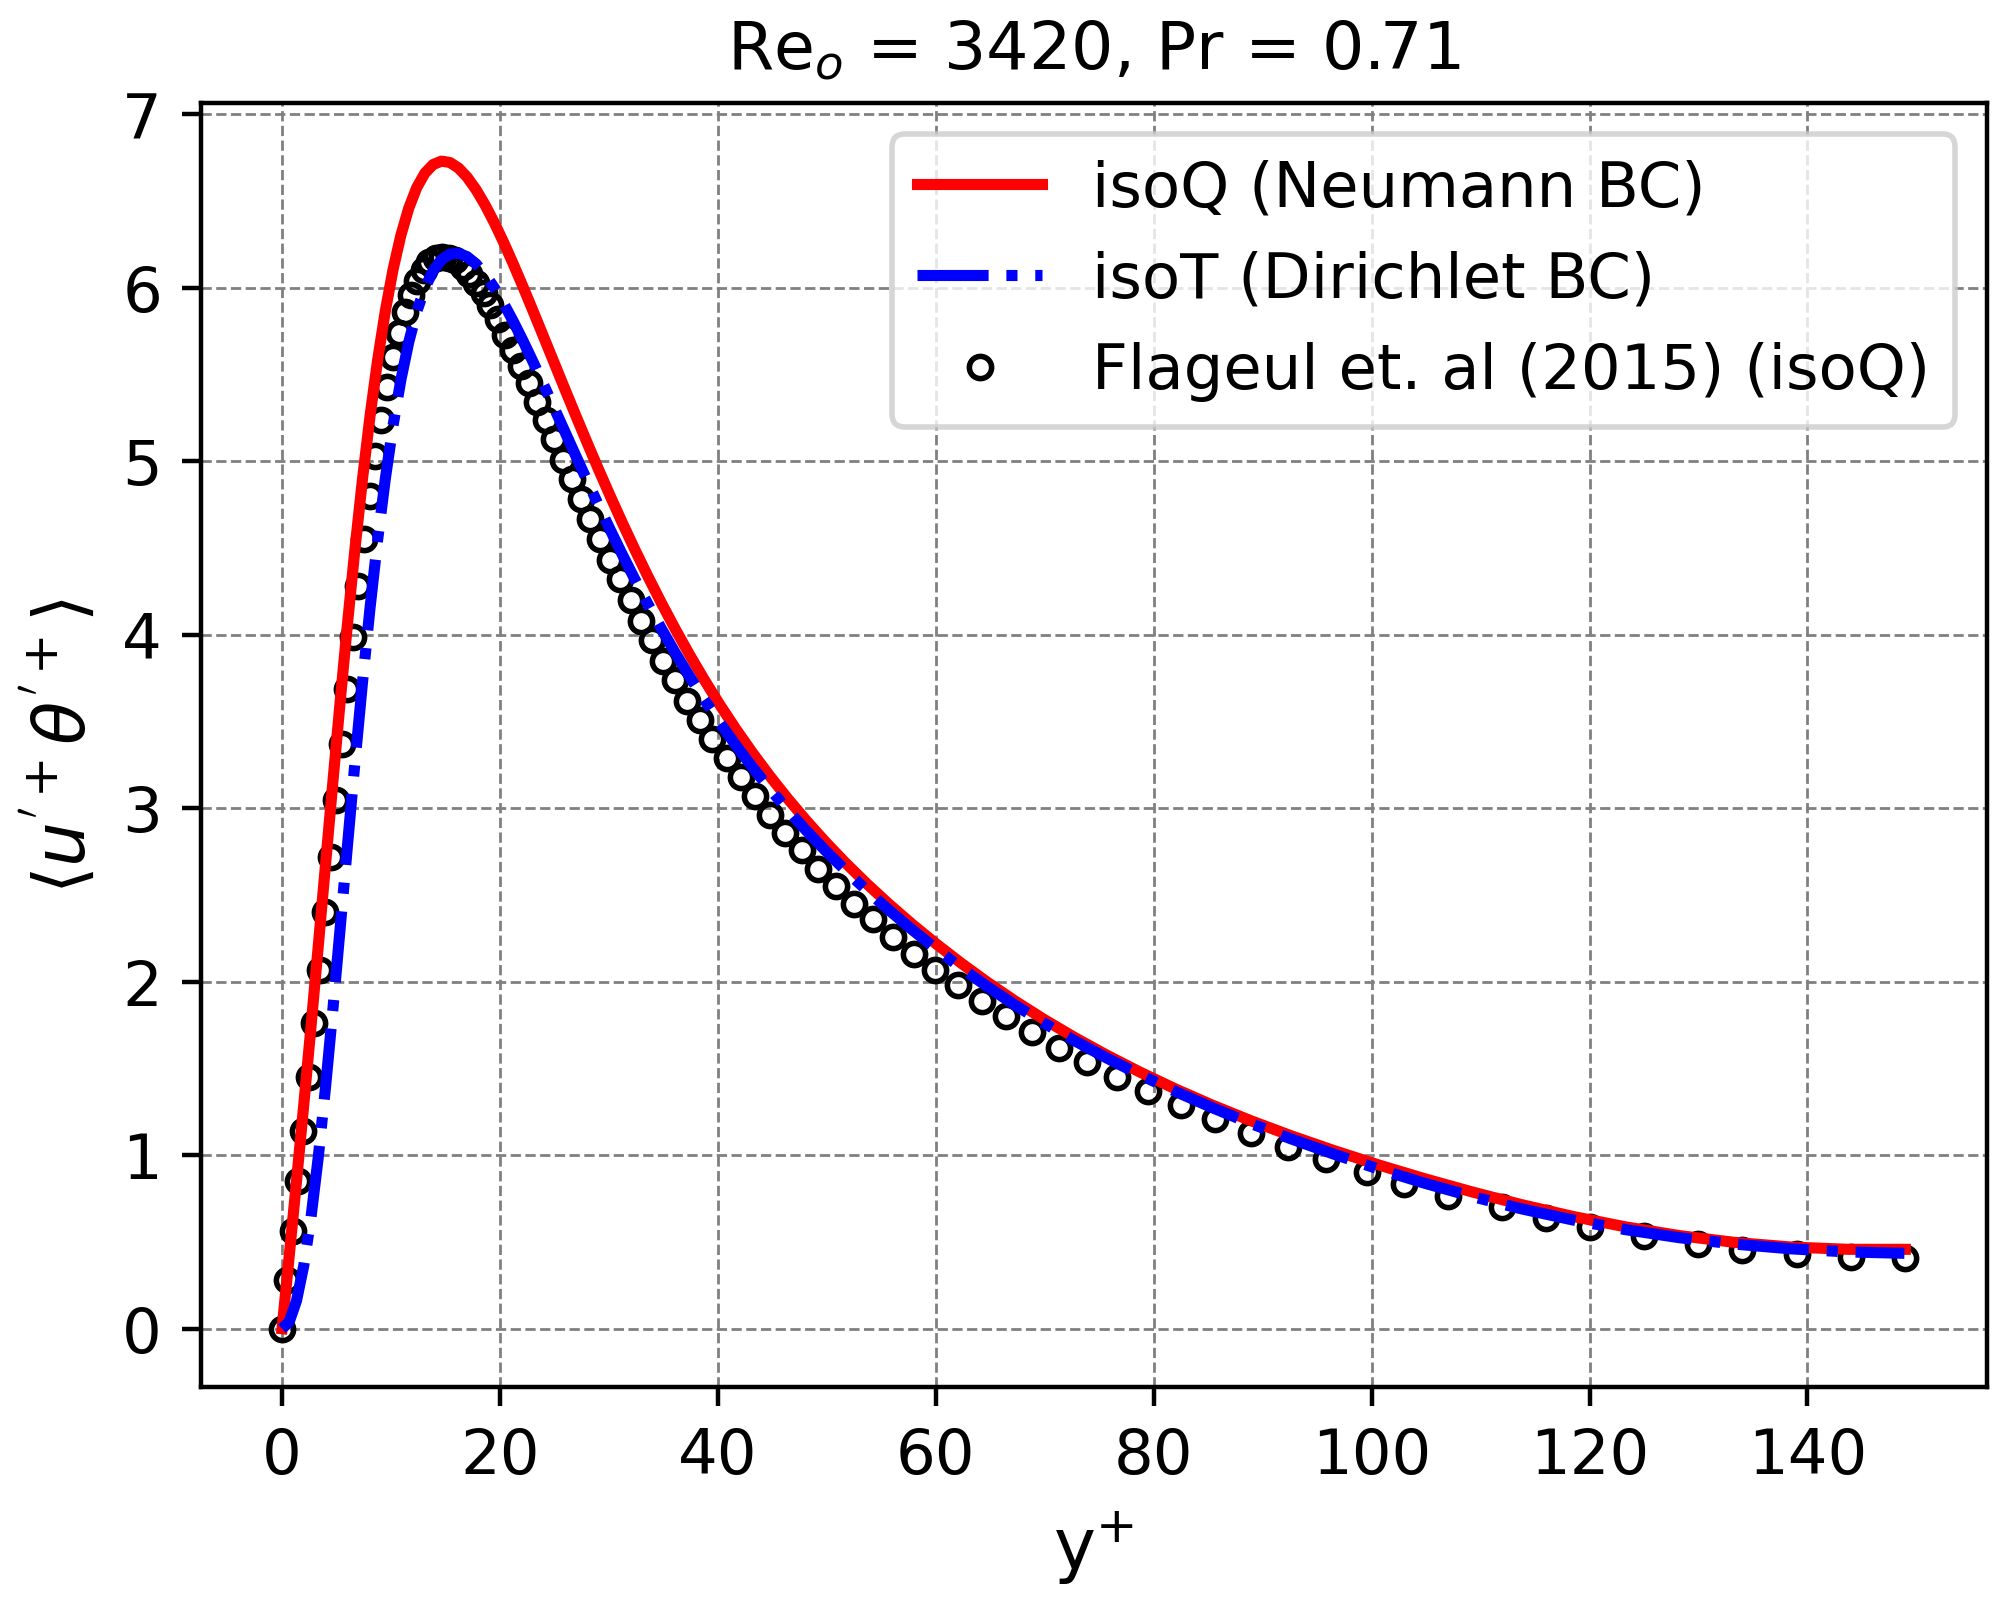
\includegraphics[width=0.49\textwidth]{figures/cap4/flageul/tep_up_thetap.png}
    \label{fig:flageul-up-thetap}
  \caption{}
  \label{fig:flageul}
\end{figure}

